

\begin{figure}[!h]
    \centering
    \resizebox{0.8\textwidth}{!}{
        \begin{tikzpicture}[mindmap,
        level 1 concept/.append style={level distance=130,sibling angle=90},
        ]
        \path[mindmap,concept color=black,text=white]
        node[concept] {Function}
        [clockwise from=0]
        child[concept color=red]{
          node[concept] (exponential) {Exponential Function}
        }
        child[concept color=blue] {
            node[concept] (inverse) {Inverse Function}
        }
        child[concept color=green!50] {
            node[concept] (logarithm) {Logarithmic Function} 
        }
        child[concept color=gray] {
            node[concept] (rangeDomain) {Range / Domain} 
        };

        \begin{pgfonlayer}{background}
        \draw [left color=red, right color=green, draw=white,
               decorate,decoration=circle connection bar] 
               (exponential) -- (logarithm);
        \draw [left color=blue, right color=red, draw=white,
               decorate,decoration=circle connection bar] 
               (exponential) -- (inverse);
        \draw [left color=green!50, right color=blue, draw=white,
               decorate,decoration=circle connection bar] 
               (logarithm) -- (inverse);
        \end{pgfonlayer}


        \end{tikzpicture}
    }
\end{figure}


%=========================================================================
% Start of
%=========================================================================
\preClass{Introduction to Exponential Functions}

\begin{problem}
\item Carbon-15 has a half life of about 2.5 seconds. If an object has
  2 grams of carbon-15 in it now, then in 2.5 seconds it will only
  have 1 gram due to its decay. An object has $8.0\times 10^-{6}$
  grams of carbon-15, and it is placed in a sealed
  container. Determine how much carbon-15 is contained in the object
  at the following times:
  \begin{subproblem}
  \item After 2.5 seconds.
    \vfill
  \item After 5.0 seconds.
    \vfill
  \item After 7.5 seconds.
    \vfill
  \item After 10.0 seconds.
    \vfill
  \end{subproblem}
\end{problem}


\actTitle{Introduction to Exponential Functions}
\begin{problem}
\item A species of bacteria is able to divide every three hours. That
  is every three hours each bacteria splits into two new
  individuals. A colony starts with 10,000 individuals. Determine the
  number of bacteria at the following times''
  \begin{subproblem}
  \item At $t=3$ hours.
    \vfill
  \item At $t=6$ hours.
    \vfill
  \item At $t=9$ hours.
    \vfill
  \item At $t=n\times 3$ hours where $n$ is an integer greater than or equal to zero.
    \vfill
  \item How many bacteria were in the colony 3 hours before the start
    of the experiment?
    \vfill
  \end{subproblem}

  \clearpage

\item A species of bacteria is able to divide every five hours. That
  is every three hours each bacteria splits into two new
  individuals. After each division, only 75\% of the remaining
  bacteria survive. A colony starts with 10,000 individuals. Determine
  the number of bacteria at the following times:
  \begin{subproblem}
  \item At $t=5$ hours.
    \vfill
  \item At $t=10$ hours.
    \vfill
  \item At $t=15$ hours.
    \vfill
  \item At $t=n\times 5$ hours where $n$ is an integer greater than zero.
    \vfill
  \item How many bacteria were in the colony 5 hours before the start
    of the experiment?
    \vfill
  \end{subproblem}

  \clearpage

\item A bank offers a savings account in which the interest is
  compounded 1.5\% annually, and the interest is accrued each
  month. If a person places \$1,000 in an account how much money is in
  the account after $n$ months?
  \textit{Determine the amount of money in the account after the
    first, second, and third months. Do not simplify your results, and
  try to find the pattern.}

  \vfill

  \clearpage

\item Simplify each expression below.
  \begin{subproblem}
  \item $\frac{3^5\cdot 3^2}{3^4}$
    \vfill
  \item $\frac{2^8}{2^5}$
    \vfill
  \item $\frac{4^2\cdot 2^2}{4^3}$
    \vfill
  \item $5^9\cdot 5^2\cdot 5^{-7}$
    \vfill
  \item $\left(\frac{1}{2}\right)^5 \cdot 2^9 \cdot 2^{-3}$
    \vfill
  \end{subproblem}

\end{problem}

\postClass

\begin{problem}
\item Briefly state two ideas from today's class.
  \begin{itemize}
  \item
  \item
  \end{itemize}
\item A bank offers 1.5\% annual interest compounded weekly (assume 52
  weeks in a year). You will deposit \$5,000 into the account. How
  much money will be in the account at any time?
\item A bank offers 1.5\% annual interest compounded monthly. You will
  deposit some money into an account and wish to have \$25,000 after
  two years. How much money should you deposit?
\item A compound is created that decays over time. It takes four years
  until half of the compound decays in a sample. You wish to store the
  compound for 5 years. How much should you store so that there will be
  4 kg of material at the end of the time period?
\end{problem}


\propertiesTitle{Properties of Exponential Functions}

Exponential functions are used whenever some quantity has a
proportional increase over fixed time spans. An example is a
bacteria population that increases by 100\% every six hours. That
means that every six hours the population doubles. In the diagram
below, a single bacteria starts in a sample. After the first time
period, six hours, there are two bacteria. After another six hours,
a total of 12 hours, there are four bacteria.
In each six hour time period that follows the population doubles.

\begin{minipage}{\linewidth}
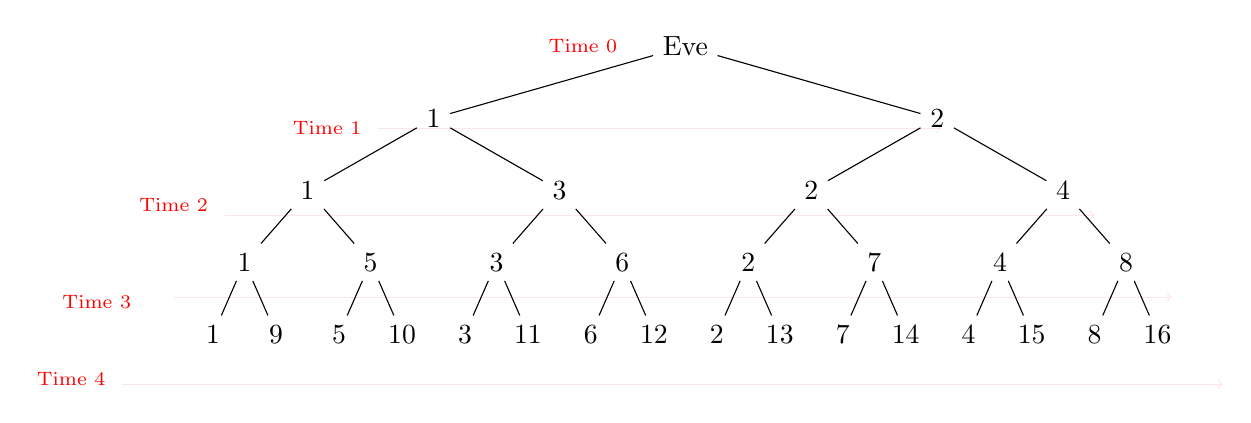
\begin{tikzpicture}[
  scale=0.65,
  grow=down,
  level 1/.style={sibling distance=28em},
  level 2/.style={sibling distance=14em},
  level 3/.style={sibling distance=7em},
  level 4/.style={sibling distance=3.5em},
  level distance = 4em
]
  \draw (-2,0) node [red] {\scriptsize Time 0};
  \draw (-7,-1.6) node [red] {\scriptsize Time 1};
  \draw [->,red!10] (-6,-1.6) -- (5,-1.6);
  \draw (-10,-3.1) node [red] {\scriptsize Time 2};
  \draw [->,red!10] (-9,-3.3) -- (8,-3.3);
  \draw (-11.5,-5.0) node [red] {\scriptsize Time 3};
  \draw [->,red!10] (-10.0,-4.9) -- (9.5,-4.9);
  \draw (-12.0,-6.5) node [red] {\scriptsize Time 4};
  \draw [->,red!10] (-11.0,-6.6) -- (10.5,-6.6);

\node{Eve} %
   child{ node {1}
     child{ node {1}
       child{ node {1}
         child{ node {1}}
         child{ node {9}}
       }
       child{ node {5}
         child{ node {5}}
         child{ node {10}}
       }
     }
     child{ node {3}
       child{ node {3}
         child{ node {3}}
         child{ node {11}}
       }
       child{ node {6}
         child{ node {6}}
         child{ node {12}}
       }
     }
   }
   child{ node {2}
     child{ node {2}
       child{ node {2}
         child{ node {2}}
         child{ node {13}}
       }
       child{ node {7}
         child{ node {7}}
         child{ node {14}}
       }
     }
     child{ node {4}
       child{ node {4}
         child{ node {4}}
         child{ node {15}}
       }
       child{ node {8}
         child{ node {8}}
         child{ node {16}}
       }
     }
   };
\end{tikzpicture}
\end{minipage}

%\clearpage
\vfill

Exponential functions satisfy the algebraic properties given below. In
each example it is assumed that $a$, $b$, and $c$ are constants, and
$a>0$.
\begin{eqnarray}
  a^b \cdot a^c & = & a^{b+c}   \\ [10pt]
  \frac{a^b}{a^c} & = & a^{b-c} \\  [10pt]
  \left( a^b \right)^c & = & a^{b\cdot c}
\end{eqnarray}

Also, $e$ is a constant number, and we define the number $e$ to be
\begin{eqnarray*}
  e & \approx & 2.718.
\end{eqnarray*}

It is common to use the number $e$ as the base for exponentials. The
number $e$ plays the same role as the constant $a$ in the equations
above:
\begin{eqnarray}
  e^b \cdot e^c & = & e^{b+c}   \\ [10pt]
  \frac{e^b}{e^c} & = & e^{b-c} \\  [10pt]
  \left( e^b \right)^c & = & e^{b\cdot c}
\end{eqnarray}



%%% Local Variables:
%%% mode: latex
%%% TeX-master: "../labManual"
%%% End:


%=========================================================================
% Start of 
%=========================================================================
\preClass{Algebra With Exponentials}

\begin{problem}
\item Determine an approximation for the value of each expression
  below. Use a calculator, and your approximation should be to the
  nearest 0.01.
  \begin{subproblem}
  \item $2^{3}$
    \vfill
  \item $2.5^{3}$
    \vfill
  \item $2.7^{3}$
    \vfill
  \item $2.718^{3}$
    \vfill
  \item $2.7183^{3}$
    \vfill
  \end{subproblem}
\end{problem}


\actTitle{The Natural Exponential}
\begin{problem}
\item A bank manager is considering the impact of different terms for
  an account that offers compounded interest. She assumes that the
  interest rate is a constant annual one percent rate and then checks
  to see what happens for different lengths of time between
  compounding. Assume that one dollar is initially deposited.
  \begin{subproblem}
  \item Determine the amount of money in the account after one hundred
    years, if the interest is compounded yearly.  \vfill
  \item Determine the amount of money in the account after 100 years,
    if the interest is compounded once every six months.  \vfill
  \item Determine the amount of money in the account after 100 years,
    if the interest is compounded once a month.
    \vfill
  \item Determine the amount of money in the account after 100 years,
    if the interest is compounded once a day.
    \vfill
  \item Determine the amount of money in the account after 100 years,
    if the interest is compounded twice  a day.
    \vfill    
  \item What is happening to the balance as the number of terms
    increases?
    \vfill
  \end{subproblem}
  \clearpage

\item Generalize the value found on the previous page.
  \begin{subproblem}
  \item Determine a formula for the balance for 1\% annual interest
    after 100 years if the interest is compounded $n$ times per year.
    \vfill
  \item Make a substitution, $u=100n$, in the previous
    expression. Write out the expression for the balance as a function
    of $u$.
    \sideNote{You can solve the substitution for $n$ if you are not
      sure how to do proceed.}
    \vfill
  \item Determine the values of the balance for the following values
    of $u$.

    \begin{tabular}{l|l}
      $u$ & balance \\ \hline
      1    &  \\ \hline
      2    &  \\ \hline
      12   &  \\ \hline
      365  &  \\ \hline
      1000 &  \\ \hline
    \end{tabular}

  \item What is the value approaching as $u$ gets large? This is a
    number that occurs in many situations, and we do not want to write
    it out every time we use it, so we use the symbol $e$ as a form of
    short hand notation.
    \begin{eqnarray*}
      e & \approx & 
    \end{eqnarray*}
    
  \end{subproblem}

  \clearpage

\item When interest is compounded continuously, the balance is
  determined using the function
  \begin{eqnarray*}
    \mathrm{Balance}(t) & = & P e^{rt},
  \end{eqnarray*}
  where $P$ is the initial balance, $r$ is the annual interest rate,
  and $t$ is the time in years.

  \begin{subproblem}
  \item Sketch a plot of the balance over time if 1\$ is deposited with a
    rate of 1\%.
    \sideNote{Label your axes and annotate your plot.}

    \vfill

  \item What happens to the balance as time increases?

    \vspace{3em}

  \item What would happen to the graph if you make $r$ bigger? What if
    $r$ is smaller?

    \vspace{3em}
  \end{subproblem}
\clearpage

\item As radioactive isotopes decay, the amount of isotope in a sample
  decreases. If the decay rate of an isotope is $r$ then the amount of
  an isotope in a sample is expressed using the function
  \begin{eqnarray*}
    \mathrm{Amount}(t) & = & A e^{-rt},
  \end{eqnarray*}
  where $t$ is measured in years.

  \begin{subproblem}
  \item What is the physical interpretation of the constant $A$?
    \vspace{2em}

  \item If a sample of a radioactive substance initially contains 3
    grams, and the radioactive decay is 0.00004, sketch a plot of the
    amount of the substance in the sample over time.
    \sideNote{Label your axes and annotate your plot. Your plot does
      not have to be perfect. Just try to get the general shape.}
    
    \vfill

  \item What happens to the amount of the radioactive substance in the
    sample as time increases?
    
    \vspace{3em}

  \item What would happen to the graph if you make $r$ bigger? What if
    $r$ is smaller?

    \vspace{3em}


  \end{subproblem}

\clearpage

\item Simplify each of the following expressions.
  \begin{subproblem}
  \item ${\displaystyle \left(e^{4.22}\right)^3}$
    \vfill
  \item ${\displaystyle e^{3.2}\cdot e^{1.8}}$
    \vfill
  \item ${\displaystyle e^{9.33}\cdot e^{t}}$
    \vfill
  \item ${\displaystyle \left(e^{4.19}\cdot e^{2t}\right)^2}$
    \vfill
  \item ${\displaystyle \left(e^{1.9}\right)^t}$
    \vfill
  \item ${\displaystyle \left(e^r\right)^t = \left( \frac{1}{2} \right)^t}$
    \vfill
  \end{subproblem}

\clearpage

\item The natural exponential function, $e^x$, is a one-to-one
  function, and it must have an inverse. Before we explore the
  function, we examine an important property of the function. The
  function is called the natural logarithm, $\ln(x)$.  In particular
  we want to examine ways to write the expression $e^a\cdot e^b$. For
  each question below, solve the relationships as requested.
  \begin{subproblem}
  \item Use the properties of the exponential to represent the product
    $e^a\cdot e^b$ as $e$ raised to a single exponential.
    \sideNote{Write the result as $e^a\cdot e^b=e^{\#}$ }
    \label{subprob:exponentialExpansion}
    \begin{eqnarray}
      \label{eqn:exponentialExpansion}
      e^a \cdot e^b & = & 
    \end{eqnarray}
    
  \item If $e^a=x$ substitute this value for $e^a$ into the left hand
    side of equation (\ref{eqn:exponentialExpansion}) above.
    
    \vspace{4em}
    
  \item If $e^b=y$ substitute this value for $e^b$ into the left hand
    side of your previous expression above.
    
    \vspace{4em}
    
  \item Take the natural logarithm of both sides of 
    the previous expression and simplify the expression.
    
    \vfill
    
  \item Solve $e^a=x$ for $a$ and solve $e^b=y$ for $b$ in the
    previous expression and substitute the result into the expression
    from above.
    
    \vfill
    
  \item What does this imply about the expression 
    \begin{eqnarray*}
      \ln\lp x \cdot y \rp & = & \hspace{10em}.
    \end{eqnarray*}
  \end{subproblem}

  \clearpage

\item We now examine another property of the inverse of the natural
  exponential, $e^x$. Recall that the inverse is denoted $\ln(x)$. In
  particular we look at the logarithm of $x^r$ where $r$ is a
  constant.
  \begin{subproblem}
  \item We can use the algebraic rule $x^r=\lp x \rp^r$. Substitute
    the identity $x=e^{\ln(x)}$ to rewrite the right side of the
    expression: \sideNote{Write the result as $x^r=\left({\#}\right)^r$ }
    \begin{eqnarray}
      \label{eqn:exponentialMultiplication}
      x^r & = & 
    \end{eqnarray}

    
    \item Expand and simplify the exponent in the right hand side of
      the expression.
      \vfill
    \item Take the logarithm of both sides of the expression. Do not
      simplify the left hand side of the expression, but simplify the
      right hand side of the expression.
      \vfill
    \item What does this imply about the expression
    \begin{eqnarray*}
      \ln\lp x^r \rp & = & \hspace{10em}.
    \end{eqnarray*}
  \end{subproblem}


\end{problem}

\postClass

\begin{problem}
\item Briefly state two ideas from today's class.
  \begin{itemize}
  \item 
  \item 
  \end{itemize}
\item The average rate of change for a function from $x=a$ to $x=b$ is
  defined to be 
  \begin{eqnarray*}
    \mathrm{Avg.~Rate~of~Change} & = & \frac{f(b)-f(a)}{b-a}.
  \end{eqnarray*}
  \scalebox{0.65}{%% Creator: Matplotlib, PGF backend
%%
%% To include the figure in your LaTeX document, write
%%   \input{<filename>.pgf}
%%
%% Make sure the required packages are loaded in your preamble
%%   \usepackage{pgf}
%%
%% Figures using additional raster images can only be included by \input if
%% they are in the same directory as the main LaTeX file. For loading figures
%% from other directories you can use the `import` package
%%   \usepackage{import}
%% and then include the figures with
%%   \import{<path to file>}{<filename>.pgf}
%%
%% Matplotlib used the following preamble
%%   \usepackage{fontspec}
%%   \setmainfont{Bitstream Vera Serif}
%%   \setsansfont{Bitstream Vera Sans}
%%   \setmonofont{Bitstream Vera Sans Mono}
%%
\begingroup%
\makeatletter%
\begin{pgfpicture}%
\pgfpathrectangle{\pgfpointorigin}{\pgfqpoint{8.000000in}{6.000000in}}%
\pgfusepath{use as bounding box, clip}%
\begin{pgfscope}%
\pgfsetbuttcap%
\pgfsetmiterjoin%
\definecolor{currentfill}{rgb}{1.000000,1.000000,1.000000}%
\pgfsetfillcolor{currentfill}%
\pgfsetlinewidth{0.000000pt}%
\definecolor{currentstroke}{rgb}{1.000000,1.000000,1.000000}%
\pgfsetstrokecolor{currentstroke}%
\pgfsetdash{}{0pt}%
\pgfpathmoveto{\pgfqpoint{0.000000in}{0.000000in}}%
\pgfpathlineto{\pgfqpoint{8.000000in}{0.000000in}}%
\pgfpathlineto{\pgfqpoint{8.000000in}{6.000000in}}%
\pgfpathlineto{\pgfqpoint{0.000000in}{6.000000in}}%
\pgfpathclose%
\pgfusepath{fill}%
\end{pgfscope}%
\begin{pgfscope}%
\pgfsetbuttcap%
\pgfsetmiterjoin%
\definecolor{currentfill}{rgb}{1.000000,1.000000,1.000000}%
\pgfsetfillcolor{currentfill}%
\pgfsetlinewidth{0.000000pt}%
\definecolor{currentstroke}{rgb}{0.000000,0.000000,0.000000}%
\pgfsetstrokecolor{currentstroke}%
\pgfsetstrokeopacity{0.000000}%
\pgfsetdash{}{0pt}%
\pgfpathmoveto{\pgfqpoint{1.000000in}{0.600000in}}%
\pgfpathlineto{\pgfqpoint{7.200000in}{0.600000in}}%
\pgfpathlineto{\pgfqpoint{7.200000in}{5.400000in}}%
\pgfpathlineto{\pgfqpoint{1.000000in}{5.400000in}}%
\pgfpathclose%
\pgfusepath{fill}%
\end{pgfscope}%
\begin{pgfscope}%
\pgfpathrectangle{\pgfqpoint{1.000000in}{0.600000in}}{\pgfqpoint{6.200000in}{4.800000in}} %
\pgfusepath{clip}%
\pgfsetbuttcap%
\pgfsetmiterjoin%
\definecolor{currentfill}{rgb}{0.000000,0.000000,0.000000}%
\pgfsetfillcolor{currentfill}%
\pgfsetlinewidth{1.003750pt}%
\definecolor{currentstroke}{rgb}{0.000000,0.000000,0.000000}%
\pgfsetstrokecolor{currentstroke}%
\pgfsetdash{}{0pt}%
\pgfpathmoveto{\pgfqpoint{4.100000in}{3.526829in}}%
\pgfpathcurveto{\pgfqpoint{4.120052in}{3.526829in}}{\pgfqpoint{4.139285in}{3.532997in}}{\pgfqpoint{4.153464in}{3.543974in}}%
\pgfpathcurveto{\pgfqpoint{4.167643in}{3.554951in}}{\pgfqpoint{4.175610in}{3.569842in}}{\pgfqpoint{4.175610in}{3.585366in}}%
\pgfpathcurveto{\pgfqpoint{4.175610in}{3.600890in}}{\pgfqpoint{4.167643in}{3.615780in}}{\pgfqpoint{4.153464in}{3.626757in}}%
\pgfpathcurveto{\pgfqpoint{4.139285in}{3.637735in}}{\pgfqpoint{4.120052in}{3.643902in}}{\pgfqpoint{4.100000in}{3.643902in}}%
\pgfpathcurveto{\pgfqpoint{4.079948in}{3.643902in}}{\pgfqpoint{4.060715in}{3.637735in}}{\pgfqpoint{4.046536in}{3.626757in}}%
\pgfpathcurveto{\pgfqpoint{4.032357in}{3.615780in}}{\pgfqpoint{4.024390in}{3.600890in}}{\pgfqpoint{4.024390in}{3.585366in}}%
\pgfpathcurveto{\pgfqpoint{4.024390in}{3.569842in}}{\pgfqpoint{4.032357in}{3.554951in}}{\pgfqpoint{4.046536in}{3.543974in}}%
\pgfpathcurveto{\pgfqpoint{4.060715in}{3.532997in}}{\pgfqpoint{4.079948in}{3.526829in}}{\pgfqpoint{4.100000in}{3.526829in}}%
\pgfpathlineto{\pgfqpoint{4.100000in}{3.526829in}}%
\pgfusepath{stroke,fill}%
\end{pgfscope}%
\begin{pgfscope}%
\pgfpathrectangle{\pgfqpoint{1.000000in}{0.600000in}}{\pgfqpoint{6.200000in}{4.800000in}} %
\pgfusepath{clip}%
\pgfsetbuttcap%
\pgfsetmiterjoin%
\definecolor{currentfill}{rgb}{0.000000,0.000000,0.000000}%
\pgfsetfillcolor{currentfill}%
\pgfsetlinewidth{1.003750pt}%
\definecolor{currentstroke}{rgb}{0.000000,0.000000,0.000000}%
\pgfsetstrokecolor{currentstroke}%
\pgfsetdash{}{0pt}%
\pgfpathmoveto{\pgfqpoint{6.368293in}{4.532653in}}%
\pgfpathcurveto{\pgfqpoint{6.388345in}{4.532653in}}{\pgfqpoint{6.407578in}{4.538821in}}{\pgfqpoint{6.421757in}{4.549798in}}%
\pgfpathcurveto{\pgfqpoint{6.435936in}{4.560775in}}{\pgfqpoint{6.443902in}{4.575665in}}{\pgfqpoint{6.443902in}{4.591189in}}%
\pgfpathcurveto{\pgfqpoint{6.443902in}{4.606713in}}{\pgfqpoint{6.435936in}{4.621604in}}{\pgfqpoint{6.421757in}{4.632581in}}%
\pgfpathcurveto{\pgfqpoint{6.407578in}{4.643558in}}{\pgfqpoint{6.388345in}{4.649726in}}{\pgfqpoint{6.368293in}{4.649726in}}%
\pgfpathcurveto{\pgfqpoint{6.348241in}{4.649726in}}{\pgfqpoint{6.329007in}{4.643558in}}{\pgfqpoint{6.314829in}{4.632581in}}%
\pgfpathcurveto{\pgfqpoint{6.300650in}{4.621604in}}{\pgfqpoint{6.292683in}{4.606713in}}{\pgfqpoint{6.292683in}{4.591189in}}%
\pgfpathcurveto{\pgfqpoint{6.292683in}{4.575665in}}{\pgfqpoint{6.300650in}{4.560775in}}{\pgfqpoint{6.314829in}{4.549798in}}%
\pgfpathcurveto{\pgfqpoint{6.329007in}{4.538821in}}{\pgfqpoint{6.348241in}{4.532653in}}{\pgfqpoint{6.368293in}{4.532653in}}%
\pgfpathlineto{\pgfqpoint{6.368293in}{4.532653in}}%
\pgfusepath{stroke,fill}%
\end{pgfscope}%
\begin{pgfscope}%
\pgfpathrectangle{\pgfqpoint{1.000000in}{0.600000in}}{\pgfqpoint{6.200000in}{4.800000in}} %
\pgfusepath{clip}%
\pgfsetrectcap%
\pgfsetroundjoin%
\pgfsetlinewidth{2.007500pt}%
\definecolor{currentstroke}{rgb}{0.000000,0.000000,0.000000}%
\pgfsetstrokecolor{currentstroke}%
\pgfsetdash{}{0pt}%
\pgfpathmoveto{\pgfqpoint{1.075610in}{3.154301in}}%
\pgfpathlineto{\pgfqpoint{1.151220in}{3.159531in}}%
\pgfpathlineto{\pgfqpoint{1.226829in}{3.164938in}}%
\pgfpathlineto{\pgfqpoint{1.302439in}{3.170529in}}%
\pgfpathlineto{\pgfqpoint{1.378049in}{3.176309in}}%
\pgfpathlineto{\pgfqpoint{1.453659in}{3.182285in}}%
\pgfpathlineto{\pgfqpoint{1.529268in}{3.188463in}}%
\pgfpathlineto{\pgfqpoint{1.604878in}{3.194851in}}%
\pgfpathlineto{\pgfqpoint{1.680488in}{3.201456in}}%
\pgfpathlineto{\pgfqpoint{1.756098in}{3.208284in}}%
\pgfpathlineto{\pgfqpoint{1.831707in}{3.215344in}}%
\pgfpathlineto{\pgfqpoint{1.907317in}{3.222643in}}%
\pgfpathlineto{\pgfqpoint{1.982927in}{3.230190in}}%
\pgfpathlineto{\pgfqpoint{2.058537in}{3.237992in}}%
\pgfpathlineto{\pgfqpoint{2.134146in}{3.246059in}}%
\pgfpathlineto{\pgfqpoint{2.209756in}{3.254399in}}%
\pgfpathlineto{\pgfqpoint{2.285366in}{3.263022in}}%
\pgfpathlineto{\pgfqpoint{2.360976in}{3.271937in}}%
\pgfpathlineto{\pgfqpoint{2.436585in}{3.281154in}}%
\pgfpathlineto{\pgfqpoint{2.512195in}{3.290684in}}%
\pgfpathlineto{\pgfqpoint{2.587805in}{3.300537in}}%
\pgfpathlineto{\pgfqpoint{2.663415in}{3.310724in}}%
\pgfpathlineto{\pgfqpoint{2.739024in}{3.321256in}}%
\pgfpathlineto{\pgfqpoint{2.814634in}{3.332145in}}%
\pgfpathlineto{\pgfqpoint{2.890244in}{3.343403in}}%
\pgfpathlineto{\pgfqpoint{2.965854in}{3.355042in}}%
\pgfpathlineto{\pgfqpoint{3.041463in}{3.367077in}}%
\pgfpathlineto{\pgfqpoint{3.117073in}{3.379519in}}%
\pgfpathlineto{\pgfqpoint{3.192683in}{3.392382in}}%
\pgfpathlineto{\pgfqpoint{3.268293in}{3.405682in}}%
\pgfpathlineto{\pgfqpoint{3.343902in}{3.419433in}}%
\pgfpathlineto{\pgfqpoint{3.419512in}{3.433650in}}%
\pgfpathlineto{\pgfqpoint{3.495122in}{3.448348in}}%
\pgfpathlineto{\pgfqpoint{3.570732in}{3.463545in}}%
\pgfpathlineto{\pgfqpoint{3.646341in}{3.479257in}}%
\pgfpathlineto{\pgfqpoint{3.721951in}{3.495501in}}%
\pgfpathlineto{\pgfqpoint{3.797561in}{3.512297in}}%
\pgfpathlineto{\pgfqpoint{3.873171in}{3.529661in}}%
\pgfpathlineto{\pgfqpoint{3.948780in}{3.547614in}}%
\pgfpathlineto{\pgfqpoint{4.024390in}{3.566175in}}%
\pgfpathlineto{\pgfqpoint{4.100000in}{3.585366in}}%
\pgfpathlineto{\pgfqpoint{4.175610in}{3.605207in}}%
\pgfpathlineto{\pgfqpoint{4.251220in}{3.625720in}}%
\pgfpathlineto{\pgfqpoint{4.326829in}{3.646929in}}%
\pgfpathlineto{\pgfqpoint{4.402439in}{3.668857in}}%
\pgfpathlineto{\pgfqpoint{4.478049in}{3.691528in}}%
\pgfpathlineto{\pgfqpoint{4.553659in}{3.714967in}}%
\pgfpathlineto{\pgfqpoint{4.629268in}{3.739201in}}%
\pgfpathlineto{\pgfqpoint{4.704878in}{3.764257in}}%
\pgfpathlineto{\pgfqpoint{4.780488in}{3.790161in}}%
\pgfpathlineto{\pgfqpoint{4.856098in}{3.816944in}}%
\pgfpathlineto{\pgfqpoint{4.931707in}{3.844634in}}%
\pgfpathlineto{\pgfqpoint{5.007317in}{3.873263in}}%
\pgfpathlineto{\pgfqpoint{5.082927in}{3.902863in}}%
\pgfpathlineto{\pgfqpoint{5.158537in}{3.933465in}}%
\pgfpathlineto{\pgfqpoint{5.234146in}{3.965105in}}%
\pgfpathlineto{\pgfqpoint{5.309756in}{3.997817in}}%
\pgfpathlineto{\pgfqpoint{5.385366in}{4.031639in}}%
\pgfpathlineto{\pgfqpoint{5.460976in}{4.066606in}}%
\pgfpathlineto{\pgfqpoint{5.536585in}{4.102759in}}%
\pgfpathlineto{\pgfqpoint{5.612195in}{4.140137in}}%
\pgfpathlineto{\pgfqpoint{5.687805in}{4.178782in}}%
\pgfpathlineto{\pgfqpoint{5.763415in}{4.218737in}}%
\pgfpathlineto{\pgfqpoint{5.839024in}{4.260046in}}%
\pgfpathlineto{\pgfqpoint{5.914634in}{4.302756in}}%
\pgfpathlineto{\pgfqpoint{5.990244in}{4.346913in}}%
\pgfpathlineto{\pgfqpoint{6.065854in}{4.392566in}}%
\pgfpathlineto{\pgfqpoint{6.141463in}{4.439768in}}%
\pgfpathlineto{\pgfqpoint{6.217073in}{4.488569in}}%
\pgfpathlineto{\pgfqpoint{6.292683in}{4.539024in}}%
\pgfpathlineto{\pgfqpoint{6.368293in}{4.591189in}}%
\pgfpathlineto{\pgfqpoint{6.443902in}{4.645123in}}%
\pgfpathlineto{\pgfqpoint{6.519512in}{4.700885in}}%
\pgfpathlineto{\pgfqpoint{6.595122in}{4.758536in}}%
\pgfpathlineto{\pgfqpoint{6.670732in}{4.818142in}}%
\pgfpathlineto{\pgfqpoint{6.746341in}{4.879768in}}%
\pgfpathlineto{\pgfqpoint{6.821951in}{4.943483in}}%
\pgfpathlineto{\pgfqpoint{6.897561in}{5.009358in}}%
\pgfpathlineto{\pgfqpoint{6.973171in}{5.077465in}}%
\pgfpathlineto{\pgfqpoint{7.048780in}{5.147881in}}%
\pgfpathlineto{\pgfqpoint{7.124390in}{5.220684in}}%
\pgfusepath{stroke}%
\end{pgfscope}%
\begin{pgfscope}%
\pgfpathrectangle{\pgfqpoint{1.000000in}{0.600000in}}{\pgfqpoint{6.200000in}{4.800000in}} %
\pgfusepath{clip}%
\pgfsetbuttcap%
\pgfsetroundjoin%
\pgfsetlinewidth{2.007500pt}%
\definecolor{currentstroke}{rgb}{0.000000,0.000000,0.000000}%
\pgfsetstrokecolor{currentstroke}%
\pgfsetdash{{6.000000pt}{6.000000pt}}{0.000000pt}%
\pgfpathmoveto{\pgfqpoint{1.075610in}{2.244268in}}%
\pgfpathlineto{\pgfqpoint{7.124390in}{4.926464in}}%
\pgfusepath{stroke}%
\end{pgfscope}%
\begin{pgfscope}%
\pgfsetrectcap%
\pgfsetmiterjoin%
\pgfsetlinewidth{0.000000pt}%
\definecolor{currentstroke}{rgb}{0.000000,0.000000,0.000000}%
\pgfsetstrokecolor{currentstroke}%
\pgfsetstrokeopacity{0.000000}%
\pgfsetdash{}{0pt}%
\pgfpathmoveto{\pgfqpoint{1.000000in}{5.400000in}}%
\pgfpathlineto{\pgfqpoint{7.200000in}{5.400000in}}%
\pgfusepath{}%
\end{pgfscope}%
\begin{pgfscope}%
\pgfsetrectcap%
\pgfsetmiterjoin%
\pgfsetlinewidth{0.000000pt}%
\definecolor{currentstroke}{rgb}{0.000000,0.000000,0.000000}%
\pgfsetstrokecolor{currentstroke}%
\pgfsetstrokeopacity{0.000000}%
\pgfsetdash{}{0pt}%
\pgfpathmoveto{\pgfqpoint{7.200000in}{0.600000in}}%
\pgfpathlineto{\pgfqpoint{7.200000in}{5.400000in}}%
\pgfusepath{}%
\end{pgfscope}%
\begin{pgfscope}%
\pgfsetrectcap%
\pgfsetmiterjoin%
\pgfsetlinewidth{1.003750pt}%
\definecolor{currentstroke}{rgb}{0.000000,0.000000,0.000000}%
\pgfsetstrokecolor{currentstroke}%
\pgfsetdash{}{0pt}%
\pgfpathmoveto{\pgfqpoint{1.000000in}{3.000000in}}%
\pgfpathlineto{\pgfqpoint{7.200000in}{3.000000in}}%
\pgfusepath{stroke}%
\end{pgfscope}%
\begin{pgfscope}%
\pgfsetrectcap%
\pgfsetmiterjoin%
\pgfsetlinewidth{1.003750pt}%
\definecolor{currentstroke}{rgb}{0.000000,0.000000,0.000000}%
\pgfsetstrokecolor{currentstroke}%
\pgfsetdash{}{0pt}%
\pgfpathmoveto{\pgfqpoint{4.100000in}{0.600000in}}%
\pgfpathlineto{\pgfqpoint{4.100000in}{5.400000in}}%
\pgfusepath{stroke}%
\end{pgfscope}%
\begin{pgfscope}%
\pgfsetbuttcap%
\pgfsetroundjoin%
\pgfsetlinewidth{0.501875pt}%
\definecolor{currentstroke}{rgb}{0.000000,0.000000,0.000000}%
\pgfsetstrokecolor{currentstroke}%
\pgfsetdash{{1.000000pt}{3.000000pt}}{0.000000pt}%
\pgfpathmoveto{\pgfqpoint{1.075610in}{0.600000in}}%
\pgfpathlineto{\pgfqpoint{1.075610in}{5.400000in}}%
\pgfusepath{stroke}%
\end{pgfscope}%
\begin{pgfscope}%
\pgfsetbuttcap%
\pgfsetroundjoin%
\definecolor{currentfill}{rgb}{0.000000,0.000000,0.000000}%
\pgfsetfillcolor{currentfill}%
\pgfsetlinewidth{0.501875pt}%
\definecolor{currentstroke}{rgb}{0.000000,0.000000,0.000000}%
\pgfsetstrokecolor{currentstroke}%
\pgfsetdash{}{0pt}%
\pgfsys@defobject{currentmarker}{\pgfqpoint{0.000000in}{0.000000in}}{\pgfqpoint{0.000000in}{0.055556in}}{%
\pgfpathmoveto{\pgfqpoint{0.000000in}{0.000000in}}%
\pgfpathlineto{\pgfqpoint{0.000000in}{0.055556in}}%
\pgfusepath{stroke,fill}%
}%
\begin{pgfscope}%
\pgfsys@transformshift{1.075610in}{3.000000in}%
\pgfsys@useobject{currentmarker}{}%
\end{pgfscope}%
\end{pgfscope}%
\begin{pgfscope}%
\pgftext[x=1.075610in,y=2.944444in,,top]{\sffamily\fontsize{12.000000}{14.400000}\selectfont \(\displaystyle -4\)}%
\end{pgfscope}%
\begin{pgfscope}%
\pgfsetbuttcap%
\pgfsetroundjoin%
\pgfsetlinewidth{0.501875pt}%
\definecolor{currentstroke}{rgb}{0.000000,0.000000,0.000000}%
\pgfsetstrokecolor{currentstroke}%
\pgfsetdash{{1.000000pt}{3.000000pt}}{0.000000pt}%
\pgfpathmoveto{\pgfqpoint{1.831707in}{0.600000in}}%
\pgfpathlineto{\pgfqpoint{1.831707in}{5.400000in}}%
\pgfusepath{stroke}%
\end{pgfscope}%
\begin{pgfscope}%
\pgfsetbuttcap%
\pgfsetroundjoin%
\definecolor{currentfill}{rgb}{0.000000,0.000000,0.000000}%
\pgfsetfillcolor{currentfill}%
\pgfsetlinewidth{0.501875pt}%
\definecolor{currentstroke}{rgb}{0.000000,0.000000,0.000000}%
\pgfsetstrokecolor{currentstroke}%
\pgfsetdash{}{0pt}%
\pgfsys@defobject{currentmarker}{\pgfqpoint{0.000000in}{0.000000in}}{\pgfqpoint{0.000000in}{0.055556in}}{%
\pgfpathmoveto{\pgfqpoint{0.000000in}{0.000000in}}%
\pgfpathlineto{\pgfqpoint{0.000000in}{0.055556in}}%
\pgfusepath{stroke,fill}%
}%
\begin{pgfscope}%
\pgfsys@transformshift{1.831707in}{3.000000in}%
\pgfsys@useobject{currentmarker}{}%
\end{pgfscope}%
\end{pgfscope}%
\begin{pgfscope}%
\pgftext[x=1.831707in,y=2.944444in,,top]{\sffamily\fontsize{12.000000}{14.400000}\selectfont \(\displaystyle -3\)}%
\end{pgfscope}%
\begin{pgfscope}%
\pgfsetbuttcap%
\pgfsetroundjoin%
\pgfsetlinewidth{0.501875pt}%
\definecolor{currentstroke}{rgb}{0.000000,0.000000,0.000000}%
\pgfsetstrokecolor{currentstroke}%
\pgfsetdash{{1.000000pt}{3.000000pt}}{0.000000pt}%
\pgfpathmoveto{\pgfqpoint{2.587805in}{0.600000in}}%
\pgfpathlineto{\pgfqpoint{2.587805in}{5.400000in}}%
\pgfusepath{stroke}%
\end{pgfscope}%
\begin{pgfscope}%
\pgfsetbuttcap%
\pgfsetroundjoin%
\definecolor{currentfill}{rgb}{0.000000,0.000000,0.000000}%
\pgfsetfillcolor{currentfill}%
\pgfsetlinewidth{0.501875pt}%
\definecolor{currentstroke}{rgb}{0.000000,0.000000,0.000000}%
\pgfsetstrokecolor{currentstroke}%
\pgfsetdash{}{0pt}%
\pgfsys@defobject{currentmarker}{\pgfqpoint{0.000000in}{0.000000in}}{\pgfqpoint{0.000000in}{0.055556in}}{%
\pgfpathmoveto{\pgfqpoint{0.000000in}{0.000000in}}%
\pgfpathlineto{\pgfqpoint{0.000000in}{0.055556in}}%
\pgfusepath{stroke,fill}%
}%
\begin{pgfscope}%
\pgfsys@transformshift{2.587805in}{3.000000in}%
\pgfsys@useobject{currentmarker}{}%
\end{pgfscope}%
\end{pgfscope}%
\begin{pgfscope}%
\pgftext[x=2.587805in,y=2.944444in,,top]{\sffamily\fontsize{12.000000}{14.400000}\selectfont \(\displaystyle -2\)}%
\end{pgfscope}%
\begin{pgfscope}%
\pgfsetbuttcap%
\pgfsetroundjoin%
\pgfsetlinewidth{0.501875pt}%
\definecolor{currentstroke}{rgb}{0.000000,0.000000,0.000000}%
\pgfsetstrokecolor{currentstroke}%
\pgfsetdash{{1.000000pt}{3.000000pt}}{0.000000pt}%
\pgfpathmoveto{\pgfqpoint{3.343902in}{0.600000in}}%
\pgfpathlineto{\pgfqpoint{3.343902in}{5.400000in}}%
\pgfusepath{stroke}%
\end{pgfscope}%
\begin{pgfscope}%
\pgfsetbuttcap%
\pgfsetroundjoin%
\definecolor{currentfill}{rgb}{0.000000,0.000000,0.000000}%
\pgfsetfillcolor{currentfill}%
\pgfsetlinewidth{0.501875pt}%
\definecolor{currentstroke}{rgb}{0.000000,0.000000,0.000000}%
\pgfsetstrokecolor{currentstroke}%
\pgfsetdash{}{0pt}%
\pgfsys@defobject{currentmarker}{\pgfqpoint{0.000000in}{0.000000in}}{\pgfqpoint{0.000000in}{0.055556in}}{%
\pgfpathmoveto{\pgfqpoint{0.000000in}{0.000000in}}%
\pgfpathlineto{\pgfqpoint{0.000000in}{0.055556in}}%
\pgfusepath{stroke,fill}%
}%
\begin{pgfscope}%
\pgfsys@transformshift{3.343902in}{3.000000in}%
\pgfsys@useobject{currentmarker}{}%
\end{pgfscope}%
\end{pgfscope}%
\begin{pgfscope}%
\pgftext[x=3.343902in,y=2.944444in,,top]{\sffamily\fontsize{12.000000}{14.400000}\selectfont \(\displaystyle -1\)}%
\end{pgfscope}%
\begin{pgfscope}%
\pgfsetbuttcap%
\pgfsetroundjoin%
\pgfsetlinewidth{0.501875pt}%
\definecolor{currentstroke}{rgb}{0.000000,0.000000,0.000000}%
\pgfsetstrokecolor{currentstroke}%
\pgfsetdash{{1.000000pt}{3.000000pt}}{0.000000pt}%
\pgfpathmoveto{\pgfqpoint{4.100000in}{0.600000in}}%
\pgfpathlineto{\pgfqpoint{4.100000in}{5.400000in}}%
\pgfusepath{stroke}%
\end{pgfscope}%
\begin{pgfscope}%
\pgfsetbuttcap%
\pgfsetroundjoin%
\definecolor{currentfill}{rgb}{0.000000,0.000000,0.000000}%
\pgfsetfillcolor{currentfill}%
\pgfsetlinewidth{0.501875pt}%
\definecolor{currentstroke}{rgb}{0.000000,0.000000,0.000000}%
\pgfsetstrokecolor{currentstroke}%
\pgfsetdash{}{0pt}%
\pgfsys@defobject{currentmarker}{\pgfqpoint{0.000000in}{0.000000in}}{\pgfqpoint{0.000000in}{0.055556in}}{%
\pgfpathmoveto{\pgfqpoint{0.000000in}{0.000000in}}%
\pgfpathlineto{\pgfqpoint{0.000000in}{0.055556in}}%
\pgfusepath{stroke,fill}%
}%
\begin{pgfscope}%
\pgfsys@transformshift{4.100000in}{3.000000in}%
\pgfsys@useobject{currentmarker}{}%
\end{pgfscope}%
\end{pgfscope}%
\begin{pgfscope}%
\pgftext[x=4.100000in,y=2.944444in,,top]{\sffamily\fontsize{12.000000}{14.400000}\selectfont \(\displaystyle 0\)}%
\end{pgfscope}%
\begin{pgfscope}%
\pgfsetbuttcap%
\pgfsetroundjoin%
\pgfsetlinewidth{0.501875pt}%
\definecolor{currentstroke}{rgb}{0.000000,0.000000,0.000000}%
\pgfsetstrokecolor{currentstroke}%
\pgfsetdash{{1.000000pt}{3.000000pt}}{0.000000pt}%
\pgfpathmoveto{\pgfqpoint{4.856098in}{0.600000in}}%
\pgfpathlineto{\pgfqpoint{4.856098in}{5.400000in}}%
\pgfusepath{stroke}%
\end{pgfscope}%
\begin{pgfscope}%
\pgfsetbuttcap%
\pgfsetroundjoin%
\definecolor{currentfill}{rgb}{0.000000,0.000000,0.000000}%
\pgfsetfillcolor{currentfill}%
\pgfsetlinewidth{0.501875pt}%
\definecolor{currentstroke}{rgb}{0.000000,0.000000,0.000000}%
\pgfsetstrokecolor{currentstroke}%
\pgfsetdash{}{0pt}%
\pgfsys@defobject{currentmarker}{\pgfqpoint{0.000000in}{0.000000in}}{\pgfqpoint{0.000000in}{0.055556in}}{%
\pgfpathmoveto{\pgfqpoint{0.000000in}{0.000000in}}%
\pgfpathlineto{\pgfqpoint{0.000000in}{0.055556in}}%
\pgfusepath{stroke,fill}%
}%
\begin{pgfscope}%
\pgfsys@transformshift{4.856098in}{3.000000in}%
\pgfsys@useobject{currentmarker}{}%
\end{pgfscope}%
\end{pgfscope}%
\begin{pgfscope}%
\pgftext[x=4.856098in,y=2.944444in,,top]{\sffamily\fontsize{12.000000}{14.400000}\selectfont \(\displaystyle 1\)}%
\end{pgfscope}%
\begin{pgfscope}%
\pgfsetbuttcap%
\pgfsetroundjoin%
\pgfsetlinewidth{0.501875pt}%
\definecolor{currentstroke}{rgb}{0.000000,0.000000,0.000000}%
\pgfsetstrokecolor{currentstroke}%
\pgfsetdash{{1.000000pt}{3.000000pt}}{0.000000pt}%
\pgfpathmoveto{\pgfqpoint{5.612195in}{0.600000in}}%
\pgfpathlineto{\pgfqpoint{5.612195in}{5.400000in}}%
\pgfusepath{stroke}%
\end{pgfscope}%
\begin{pgfscope}%
\pgfsetbuttcap%
\pgfsetroundjoin%
\definecolor{currentfill}{rgb}{0.000000,0.000000,0.000000}%
\pgfsetfillcolor{currentfill}%
\pgfsetlinewidth{0.501875pt}%
\definecolor{currentstroke}{rgb}{0.000000,0.000000,0.000000}%
\pgfsetstrokecolor{currentstroke}%
\pgfsetdash{}{0pt}%
\pgfsys@defobject{currentmarker}{\pgfqpoint{0.000000in}{0.000000in}}{\pgfqpoint{0.000000in}{0.055556in}}{%
\pgfpathmoveto{\pgfqpoint{0.000000in}{0.000000in}}%
\pgfpathlineto{\pgfqpoint{0.000000in}{0.055556in}}%
\pgfusepath{stroke,fill}%
}%
\begin{pgfscope}%
\pgfsys@transformshift{5.612195in}{3.000000in}%
\pgfsys@useobject{currentmarker}{}%
\end{pgfscope}%
\end{pgfscope}%
\begin{pgfscope}%
\pgftext[x=5.612195in,y=2.944444in,,top]{\sffamily\fontsize{12.000000}{14.400000}\selectfont \(\displaystyle 2\)}%
\end{pgfscope}%
\begin{pgfscope}%
\pgfsetbuttcap%
\pgfsetroundjoin%
\pgfsetlinewidth{0.501875pt}%
\definecolor{currentstroke}{rgb}{0.000000,0.000000,0.000000}%
\pgfsetstrokecolor{currentstroke}%
\pgfsetdash{{1.000000pt}{3.000000pt}}{0.000000pt}%
\pgfpathmoveto{\pgfqpoint{6.368293in}{0.600000in}}%
\pgfpathlineto{\pgfqpoint{6.368293in}{5.400000in}}%
\pgfusepath{stroke}%
\end{pgfscope}%
\begin{pgfscope}%
\pgfsetbuttcap%
\pgfsetroundjoin%
\definecolor{currentfill}{rgb}{0.000000,0.000000,0.000000}%
\pgfsetfillcolor{currentfill}%
\pgfsetlinewidth{0.501875pt}%
\definecolor{currentstroke}{rgb}{0.000000,0.000000,0.000000}%
\pgfsetstrokecolor{currentstroke}%
\pgfsetdash{}{0pt}%
\pgfsys@defobject{currentmarker}{\pgfqpoint{0.000000in}{0.000000in}}{\pgfqpoint{0.000000in}{0.055556in}}{%
\pgfpathmoveto{\pgfqpoint{0.000000in}{0.000000in}}%
\pgfpathlineto{\pgfqpoint{0.000000in}{0.055556in}}%
\pgfusepath{stroke,fill}%
}%
\begin{pgfscope}%
\pgfsys@transformshift{6.368293in}{3.000000in}%
\pgfsys@useobject{currentmarker}{}%
\end{pgfscope}%
\end{pgfscope}%
\begin{pgfscope}%
\pgftext[x=6.368293in,y=2.944444in,,top]{\sffamily\fontsize{12.000000}{14.400000}\selectfont \(\displaystyle 3\)}%
\end{pgfscope}%
\begin{pgfscope}%
\pgfsetbuttcap%
\pgfsetroundjoin%
\pgfsetlinewidth{0.501875pt}%
\definecolor{currentstroke}{rgb}{0.000000,0.000000,0.000000}%
\pgfsetstrokecolor{currentstroke}%
\pgfsetdash{{1.000000pt}{3.000000pt}}{0.000000pt}%
\pgfpathmoveto{\pgfqpoint{7.124390in}{0.600000in}}%
\pgfpathlineto{\pgfqpoint{7.124390in}{5.400000in}}%
\pgfusepath{stroke}%
\end{pgfscope}%
\begin{pgfscope}%
\pgfsetbuttcap%
\pgfsetroundjoin%
\definecolor{currentfill}{rgb}{0.000000,0.000000,0.000000}%
\pgfsetfillcolor{currentfill}%
\pgfsetlinewidth{0.501875pt}%
\definecolor{currentstroke}{rgb}{0.000000,0.000000,0.000000}%
\pgfsetstrokecolor{currentstroke}%
\pgfsetdash{}{0pt}%
\pgfsys@defobject{currentmarker}{\pgfqpoint{0.000000in}{0.000000in}}{\pgfqpoint{0.000000in}{0.055556in}}{%
\pgfpathmoveto{\pgfqpoint{0.000000in}{0.000000in}}%
\pgfpathlineto{\pgfqpoint{0.000000in}{0.055556in}}%
\pgfusepath{stroke,fill}%
}%
\begin{pgfscope}%
\pgfsys@transformshift{7.124390in}{3.000000in}%
\pgfsys@useobject{currentmarker}{}%
\end{pgfscope}%
\end{pgfscope}%
\begin{pgfscope}%
\pgftext[x=7.124390in,y=2.944444in,,top]{\sffamily\fontsize{12.000000}{14.400000}\selectfont \(\displaystyle 4\)}%
\end{pgfscope}%
\begin{pgfscope}%
\pgftext[x=6.890000in,y=2.760000in,,top]{\sffamily\fontsize{12.000000}{14.400000}\selectfont x}%
\end{pgfscope}%
\begin{pgfscope}%
\pgfsetbuttcap%
\pgfsetroundjoin%
\pgfsetlinewidth{0.501875pt}%
\definecolor{currentstroke}{rgb}{0.000000,0.000000,0.000000}%
\pgfsetstrokecolor{currentstroke}%
\pgfsetdash{{1.000000pt}{3.000000pt}}{0.000000pt}%
\pgfpathmoveto{\pgfqpoint{1.000000in}{0.658537in}}%
\pgfpathlineto{\pgfqpoint{7.200000in}{0.658537in}}%
\pgfusepath{stroke}%
\end{pgfscope}%
\begin{pgfscope}%
\pgfsetbuttcap%
\pgfsetroundjoin%
\definecolor{currentfill}{rgb}{0.000000,0.000000,0.000000}%
\pgfsetfillcolor{currentfill}%
\pgfsetlinewidth{0.501875pt}%
\definecolor{currentstroke}{rgb}{0.000000,0.000000,0.000000}%
\pgfsetstrokecolor{currentstroke}%
\pgfsetdash{}{0pt}%
\pgfsys@defobject{currentmarker}{\pgfqpoint{0.000000in}{0.000000in}}{\pgfqpoint{0.055556in}{0.000000in}}{%
\pgfpathmoveto{\pgfqpoint{0.000000in}{0.000000in}}%
\pgfpathlineto{\pgfqpoint{0.055556in}{0.000000in}}%
\pgfusepath{stroke,fill}%
}%
\begin{pgfscope}%
\pgfsys@transformshift{4.100000in}{0.658537in}%
\pgfsys@useobject{currentmarker}{}%
\end{pgfscope}%
\end{pgfscope}%
\begin{pgfscope}%
\pgftext[x=4.044444in,y=0.658537in,right,]{\sffamily\fontsize{12.000000}{14.400000}\selectfont \(\displaystyle -4\)}%
\end{pgfscope}%
\begin{pgfscope}%
\pgfsetbuttcap%
\pgfsetroundjoin%
\pgfsetlinewidth{0.501875pt}%
\definecolor{currentstroke}{rgb}{0.000000,0.000000,0.000000}%
\pgfsetstrokecolor{currentstroke}%
\pgfsetdash{{1.000000pt}{3.000000pt}}{0.000000pt}%
\pgfpathmoveto{\pgfqpoint{1.000000in}{1.243902in}}%
\pgfpathlineto{\pgfqpoint{7.200000in}{1.243902in}}%
\pgfusepath{stroke}%
\end{pgfscope}%
\begin{pgfscope}%
\pgfsetbuttcap%
\pgfsetroundjoin%
\definecolor{currentfill}{rgb}{0.000000,0.000000,0.000000}%
\pgfsetfillcolor{currentfill}%
\pgfsetlinewidth{0.501875pt}%
\definecolor{currentstroke}{rgb}{0.000000,0.000000,0.000000}%
\pgfsetstrokecolor{currentstroke}%
\pgfsetdash{}{0pt}%
\pgfsys@defobject{currentmarker}{\pgfqpoint{0.000000in}{0.000000in}}{\pgfqpoint{0.055556in}{0.000000in}}{%
\pgfpathmoveto{\pgfqpoint{0.000000in}{0.000000in}}%
\pgfpathlineto{\pgfqpoint{0.055556in}{0.000000in}}%
\pgfusepath{stroke,fill}%
}%
\begin{pgfscope}%
\pgfsys@transformshift{4.100000in}{1.243902in}%
\pgfsys@useobject{currentmarker}{}%
\end{pgfscope}%
\end{pgfscope}%
\begin{pgfscope}%
\pgftext[x=4.044444in,y=1.243902in,right,]{\sffamily\fontsize{12.000000}{14.400000}\selectfont \(\displaystyle -3\)}%
\end{pgfscope}%
\begin{pgfscope}%
\pgfsetbuttcap%
\pgfsetroundjoin%
\pgfsetlinewidth{0.501875pt}%
\definecolor{currentstroke}{rgb}{0.000000,0.000000,0.000000}%
\pgfsetstrokecolor{currentstroke}%
\pgfsetdash{{1.000000pt}{3.000000pt}}{0.000000pt}%
\pgfpathmoveto{\pgfqpoint{1.000000in}{1.829268in}}%
\pgfpathlineto{\pgfqpoint{7.200000in}{1.829268in}}%
\pgfusepath{stroke}%
\end{pgfscope}%
\begin{pgfscope}%
\pgfsetbuttcap%
\pgfsetroundjoin%
\definecolor{currentfill}{rgb}{0.000000,0.000000,0.000000}%
\pgfsetfillcolor{currentfill}%
\pgfsetlinewidth{0.501875pt}%
\definecolor{currentstroke}{rgb}{0.000000,0.000000,0.000000}%
\pgfsetstrokecolor{currentstroke}%
\pgfsetdash{}{0pt}%
\pgfsys@defobject{currentmarker}{\pgfqpoint{0.000000in}{0.000000in}}{\pgfqpoint{0.055556in}{0.000000in}}{%
\pgfpathmoveto{\pgfqpoint{0.000000in}{0.000000in}}%
\pgfpathlineto{\pgfqpoint{0.055556in}{0.000000in}}%
\pgfusepath{stroke,fill}%
}%
\begin{pgfscope}%
\pgfsys@transformshift{4.100000in}{1.829268in}%
\pgfsys@useobject{currentmarker}{}%
\end{pgfscope}%
\end{pgfscope}%
\begin{pgfscope}%
\pgftext[x=4.044444in,y=1.829268in,right,]{\sffamily\fontsize{12.000000}{14.400000}\selectfont \(\displaystyle -2\)}%
\end{pgfscope}%
\begin{pgfscope}%
\pgfsetbuttcap%
\pgfsetroundjoin%
\pgfsetlinewidth{0.501875pt}%
\definecolor{currentstroke}{rgb}{0.000000,0.000000,0.000000}%
\pgfsetstrokecolor{currentstroke}%
\pgfsetdash{{1.000000pt}{3.000000pt}}{0.000000pt}%
\pgfpathmoveto{\pgfqpoint{1.000000in}{2.414634in}}%
\pgfpathlineto{\pgfqpoint{7.200000in}{2.414634in}}%
\pgfusepath{stroke}%
\end{pgfscope}%
\begin{pgfscope}%
\pgfsetbuttcap%
\pgfsetroundjoin%
\definecolor{currentfill}{rgb}{0.000000,0.000000,0.000000}%
\pgfsetfillcolor{currentfill}%
\pgfsetlinewidth{0.501875pt}%
\definecolor{currentstroke}{rgb}{0.000000,0.000000,0.000000}%
\pgfsetstrokecolor{currentstroke}%
\pgfsetdash{}{0pt}%
\pgfsys@defobject{currentmarker}{\pgfqpoint{0.000000in}{0.000000in}}{\pgfqpoint{0.055556in}{0.000000in}}{%
\pgfpathmoveto{\pgfqpoint{0.000000in}{0.000000in}}%
\pgfpathlineto{\pgfqpoint{0.055556in}{0.000000in}}%
\pgfusepath{stroke,fill}%
}%
\begin{pgfscope}%
\pgfsys@transformshift{4.100000in}{2.414634in}%
\pgfsys@useobject{currentmarker}{}%
\end{pgfscope}%
\end{pgfscope}%
\begin{pgfscope}%
\pgftext[x=4.044444in,y=2.414634in,right,]{\sffamily\fontsize{12.000000}{14.400000}\selectfont \(\displaystyle -1\)}%
\end{pgfscope}%
\begin{pgfscope}%
\pgfsetbuttcap%
\pgfsetroundjoin%
\pgfsetlinewidth{0.501875pt}%
\definecolor{currentstroke}{rgb}{0.000000,0.000000,0.000000}%
\pgfsetstrokecolor{currentstroke}%
\pgfsetdash{{1.000000pt}{3.000000pt}}{0.000000pt}%
\pgfpathmoveto{\pgfqpoint{1.000000in}{3.000000in}}%
\pgfpathlineto{\pgfqpoint{7.200000in}{3.000000in}}%
\pgfusepath{stroke}%
\end{pgfscope}%
\begin{pgfscope}%
\pgfsetbuttcap%
\pgfsetroundjoin%
\definecolor{currentfill}{rgb}{0.000000,0.000000,0.000000}%
\pgfsetfillcolor{currentfill}%
\pgfsetlinewidth{0.501875pt}%
\definecolor{currentstroke}{rgb}{0.000000,0.000000,0.000000}%
\pgfsetstrokecolor{currentstroke}%
\pgfsetdash{}{0pt}%
\pgfsys@defobject{currentmarker}{\pgfqpoint{0.000000in}{0.000000in}}{\pgfqpoint{0.055556in}{0.000000in}}{%
\pgfpathmoveto{\pgfqpoint{0.000000in}{0.000000in}}%
\pgfpathlineto{\pgfqpoint{0.055556in}{0.000000in}}%
\pgfusepath{stroke,fill}%
}%
\begin{pgfscope}%
\pgfsys@transformshift{4.100000in}{3.000000in}%
\pgfsys@useobject{currentmarker}{}%
\end{pgfscope}%
\end{pgfscope}%
\begin{pgfscope}%
\pgftext[x=4.044444in,y=3.000000in,right,]{\sffamily\fontsize{12.000000}{14.400000}\selectfont \(\displaystyle 0\)}%
\end{pgfscope}%
\begin{pgfscope}%
\pgfsetbuttcap%
\pgfsetroundjoin%
\pgfsetlinewidth{0.501875pt}%
\definecolor{currentstroke}{rgb}{0.000000,0.000000,0.000000}%
\pgfsetstrokecolor{currentstroke}%
\pgfsetdash{{1.000000pt}{3.000000pt}}{0.000000pt}%
\pgfpathmoveto{\pgfqpoint{1.000000in}{3.585366in}}%
\pgfpathlineto{\pgfqpoint{7.200000in}{3.585366in}}%
\pgfusepath{stroke}%
\end{pgfscope}%
\begin{pgfscope}%
\pgfsetbuttcap%
\pgfsetroundjoin%
\definecolor{currentfill}{rgb}{0.000000,0.000000,0.000000}%
\pgfsetfillcolor{currentfill}%
\pgfsetlinewidth{0.501875pt}%
\definecolor{currentstroke}{rgb}{0.000000,0.000000,0.000000}%
\pgfsetstrokecolor{currentstroke}%
\pgfsetdash{}{0pt}%
\pgfsys@defobject{currentmarker}{\pgfqpoint{0.000000in}{0.000000in}}{\pgfqpoint{0.055556in}{0.000000in}}{%
\pgfpathmoveto{\pgfqpoint{0.000000in}{0.000000in}}%
\pgfpathlineto{\pgfqpoint{0.055556in}{0.000000in}}%
\pgfusepath{stroke,fill}%
}%
\begin{pgfscope}%
\pgfsys@transformshift{4.100000in}{3.585366in}%
\pgfsys@useobject{currentmarker}{}%
\end{pgfscope}%
\end{pgfscope}%
\begin{pgfscope}%
\pgftext[x=4.044444in,y=3.585366in,right,]{\sffamily\fontsize{12.000000}{14.400000}\selectfont \(\displaystyle 1\)}%
\end{pgfscope}%
\begin{pgfscope}%
\pgfsetbuttcap%
\pgfsetroundjoin%
\pgfsetlinewidth{0.501875pt}%
\definecolor{currentstroke}{rgb}{0.000000,0.000000,0.000000}%
\pgfsetstrokecolor{currentstroke}%
\pgfsetdash{{1.000000pt}{3.000000pt}}{0.000000pt}%
\pgfpathmoveto{\pgfqpoint{1.000000in}{4.170732in}}%
\pgfpathlineto{\pgfqpoint{7.200000in}{4.170732in}}%
\pgfusepath{stroke}%
\end{pgfscope}%
\begin{pgfscope}%
\pgfsetbuttcap%
\pgfsetroundjoin%
\definecolor{currentfill}{rgb}{0.000000,0.000000,0.000000}%
\pgfsetfillcolor{currentfill}%
\pgfsetlinewidth{0.501875pt}%
\definecolor{currentstroke}{rgb}{0.000000,0.000000,0.000000}%
\pgfsetstrokecolor{currentstroke}%
\pgfsetdash{}{0pt}%
\pgfsys@defobject{currentmarker}{\pgfqpoint{0.000000in}{0.000000in}}{\pgfqpoint{0.055556in}{0.000000in}}{%
\pgfpathmoveto{\pgfqpoint{0.000000in}{0.000000in}}%
\pgfpathlineto{\pgfqpoint{0.055556in}{0.000000in}}%
\pgfusepath{stroke,fill}%
}%
\begin{pgfscope}%
\pgfsys@transformshift{4.100000in}{4.170732in}%
\pgfsys@useobject{currentmarker}{}%
\end{pgfscope}%
\end{pgfscope}%
\begin{pgfscope}%
\pgftext[x=4.044444in,y=4.170732in,right,]{\sffamily\fontsize{12.000000}{14.400000}\selectfont \(\displaystyle 2\)}%
\end{pgfscope}%
\begin{pgfscope}%
\pgfsetbuttcap%
\pgfsetroundjoin%
\pgfsetlinewidth{0.501875pt}%
\definecolor{currentstroke}{rgb}{0.000000,0.000000,0.000000}%
\pgfsetstrokecolor{currentstroke}%
\pgfsetdash{{1.000000pt}{3.000000pt}}{0.000000pt}%
\pgfpathmoveto{\pgfqpoint{1.000000in}{4.756098in}}%
\pgfpathlineto{\pgfqpoint{7.200000in}{4.756098in}}%
\pgfusepath{stroke}%
\end{pgfscope}%
\begin{pgfscope}%
\pgfsetbuttcap%
\pgfsetroundjoin%
\definecolor{currentfill}{rgb}{0.000000,0.000000,0.000000}%
\pgfsetfillcolor{currentfill}%
\pgfsetlinewidth{0.501875pt}%
\definecolor{currentstroke}{rgb}{0.000000,0.000000,0.000000}%
\pgfsetstrokecolor{currentstroke}%
\pgfsetdash{}{0pt}%
\pgfsys@defobject{currentmarker}{\pgfqpoint{0.000000in}{0.000000in}}{\pgfqpoint{0.055556in}{0.000000in}}{%
\pgfpathmoveto{\pgfqpoint{0.000000in}{0.000000in}}%
\pgfpathlineto{\pgfqpoint{0.055556in}{0.000000in}}%
\pgfusepath{stroke,fill}%
}%
\begin{pgfscope}%
\pgfsys@transformshift{4.100000in}{4.756098in}%
\pgfsys@useobject{currentmarker}{}%
\end{pgfscope}%
\end{pgfscope}%
\begin{pgfscope}%
\pgftext[x=4.044444in,y=4.756098in,right,]{\sffamily\fontsize{12.000000}{14.400000}\selectfont \(\displaystyle 3\)}%
\end{pgfscope}%
\begin{pgfscope}%
\pgfsetbuttcap%
\pgfsetroundjoin%
\pgfsetlinewidth{0.501875pt}%
\definecolor{currentstroke}{rgb}{0.000000,0.000000,0.000000}%
\pgfsetstrokecolor{currentstroke}%
\pgfsetdash{{1.000000pt}{3.000000pt}}{0.000000pt}%
\pgfpathmoveto{\pgfqpoint{1.000000in}{5.341463in}}%
\pgfpathlineto{\pgfqpoint{7.200000in}{5.341463in}}%
\pgfusepath{stroke}%
\end{pgfscope}%
\begin{pgfscope}%
\pgfsetbuttcap%
\pgfsetroundjoin%
\definecolor{currentfill}{rgb}{0.000000,0.000000,0.000000}%
\pgfsetfillcolor{currentfill}%
\pgfsetlinewidth{0.501875pt}%
\definecolor{currentstroke}{rgb}{0.000000,0.000000,0.000000}%
\pgfsetstrokecolor{currentstroke}%
\pgfsetdash{}{0pt}%
\pgfsys@defobject{currentmarker}{\pgfqpoint{0.000000in}{0.000000in}}{\pgfqpoint{0.055556in}{0.000000in}}{%
\pgfpathmoveto{\pgfqpoint{0.000000in}{0.000000in}}%
\pgfpathlineto{\pgfqpoint{0.055556in}{0.000000in}}%
\pgfusepath{stroke,fill}%
}%
\begin{pgfscope}%
\pgfsys@transformshift{4.100000in}{5.341463in}%
\pgfsys@useobject{currentmarker}{}%
\end{pgfscope}%
\end{pgfscope}%
\begin{pgfscope}%
\pgftext[x=4.044444in,y=5.341463in,right,]{\sffamily\fontsize{12.000000}{14.400000}\selectfont \(\displaystyle 4\)}%
\end{pgfscope}%
\begin{pgfscope}%
\pgftext[x=3.790000in,y=5.160000in,,bottom,rotate=90.000000]{\sffamily\fontsize{12.000000}{14.400000}\selectfont f}%
\end{pgfscope}%
\begin{pgfscope}%
\pgftext[x=4.100000in,y=5.469444in,,base]{\sffamily\fontsize{14.400000}{17.280000}\selectfont Graph of f}%
\end{pgfscope}%
\end{pgfpicture}%
\makeatother%
\endgroup%
}

  Visually, it can be thought of as the slope of the line that goes
  through the graph of the function at two points, $(a,f(a))$ and
  $(b,f(b))$.

  \begin{subproblem}
  \item The population of a colony of bacteria is two times its
    previous population every one hour. Determine the average rate of
    change from $a=0$ to the times
    given in the table below. \\
    \begin{tabular}{p{4em}|p{3em}|p{3em}|p{3em}|p{3em}|p{3em}|p{3em}}
      $b$ & 1 & $\frac{1}{2}$ & $\frac{1}{2^2}$ & $\frac{1}{2^3}$ &
      $\frac{1}{2^4}$ & $\frac{1}{2^5}$ \\ \hline
      Number Bacteria &&&&&  \\ [12pt] \hline 
      Avg Rate Change &&&&& 
    \end{tabular}

    What number is the average rate of change approaching as $b$ gets
    close to zero?

  \item The population of a colony of bacteria is three times its
    previous population every one hour. Determine the average rate of
    change from $a=0$ to the times
    given in the table below. \\
    \begin{tabular}{p{4em}|p{3em}|p{3em}|p{3em}|p{3em}|p{3em}|p{3em}}
      $b$ & 1 & $\frac{1}{2}$ & $\frac{1}{2^2}$ & $\frac{1}{2^3}$ &
      $\frac{1}{2^4}$ & $\frac{1}{2^5}$ \\ \hline
      Number Bacteria &&&&&  \\ [12pt] \hline
      Avg Rate Change &&&&& 
    \end{tabular}

    What number is the average rate of change approaching as $b$ gets
    close to zero?

  \item The population of a colony of bacteria is 2.5 its previous
    population every one hour. Determine the average rate of change
    from $a=0$ to
    the times   given in the table below. \\
    \begin{tabular}{p{4em}|p{3em}|p{3em}|p{3em}|p{3em}|p{3em}|p{3em}}
      $b$ & 1 & $\frac{1}{2}$ & $\frac{1}{2^2}$ & $\frac{1}{2^3}$ &
      $\frac{1}{2^4}$ & $\frac{1}{2^5}$ \\ \hline
      Number Bacteria &&&&&  \\ [12pt] \hline
      Avg Rate Change &&&&&
    \end{tabular}

    What number is the average rate of change approaching as $b$ gets
    close to zero?

  \item The population of a colony of bacteria is 2.7 its previous
    population every one hour. Determine the average rate of change
    from $a=0$ to
    the times   given in the table below. \\
    \begin{tabular}{p{4em}|p{3em}|p{3em}|p{3em}|p{3em}|p{3em}|p{3em}}
      $b$ & 1 & $\frac{1}{2}$ & $\frac{1}{2^2}$ & $\frac{1}{2^3}$ &
      $\frac{1}{2^4}$ & $\frac{1}{2^5}$ \\ \hline
      Number Bacteria &&&&&  \\ [12pt] \hline
      Avg Rate Change &&&&&
    \end{tabular}

    What number is the average rate of change approaching as $b$ gets
    close to zero?

  \item Determine a value so that if a population multiplies its
    population by that number every hour the average rate of change
    approaches 1 from $a=0$ and $b$ gets close to zero.

  \end{subproblem}

\end{problem}


%%% Local Variables:
%%% mode: latex
%%% TeX-master: "../labManual"
%%% End:



%=========================================================================
% Start of 
%=========================================================================
\preClass{Introduction to Logarithms}

\begin{problem}
\item A computer virus is constructed that will infect two new
  computer systems each day and then wipe the disk drive of its
  current computer clean.  The virus is installed on one computer on
  1 January.
  \begin{subproblem}
  \item How many new computers will it infect on 2 January?
    \vfill
  \item How many new computers will it infect on 3 January?
    \vfill
  \item How many new computers will it infect on 4 January?
    \vfill
  \end{subproblem}
\item A computer virus is constructed that will infect two new
  computer systems each day and then wipe the disk drive of its
  current computer clean.  The virus is installed on a computer but it
  is not clear when it was first installed.
  \begin{subproblem}
  \item It is estimated that 128 computers were infected on a given
    day. How many days beforehand was it installed on the first computer?
    \vfill
  \item It is estimated that 1024 computers were infected on a given
    day. How many days beforehand was it installed on the first computer?
    \vfill
  \item It is estimated that 32768 computers were infected on a given
    day. How many days beforehand was it installed on the first computer?
    \vfill
  \end{subproblem}
\item Make a sketch of the number line. Mark zero on your number
  line. Indicate the locations of 1, 1.5, -0.5, and 9.5. Try to make a
  good approximation of the relative distances.
\end{problem}


\actTitle{Introduction to Logarithms}
\begin{problem}
\item The approximate distances in kilometers from the earth to
  various destinations is given in the table below. Use this
  information to answer each of the questions below.

  \begin{tabular}{ll}
    Destination & Distance \\ \hline
    The moon & $3.84 \times 10^5$ km \\
    Mars &  $5.46 \times 10^7$ km \\
    Saturn & $1.28 \times 10^9$ km \\
    Proxima Centauri (Closest star) & $4.01 \times 10^{13}$ km \\
    Center of the Milky Way & $2.83 \times 10^{17}$ km
  \end{tabular}

  \begin{subproblem}
    \item Make a sketch of a number line with the distances for each
      destination marked on the number line.
      \vfill
    \item For each distance in the table above what is the approximate
      power of ten for the distance? For example, if a distance is
      $1\times 10^4$ km it is a power of 4. Sketch a number line and
      indicate the powers of ten on the number line.
      \vfill
  \end{subproblem}

\clearpage

The approximate average lengths of various items are given in the table
below. Use this information to answer each of the questions below.

  \begin{tabular}{ll}
    Item & Size \\ \hline
    Person & 1.75 m \\
    Finger & $9.2 \times 10^{-2}$ m\\
    DNA & $ 5.0 \times 10^{-2}$ m \\
    Hair (Width) & $ 9.0\times 10^{-5}$ m \\
    Bacteria & $ 0.8 \times 10^{-7}$ m\\
  \end{tabular}

  \begin{subproblem}
    \item Make a sketch of a number line with the lengths for each
      item  marked on the number line.
      \vfill
    \item For each item in the table above what is the approximate
      power of ten for the length? For example, if a length is
      $1\times 10^{-4}$ m it is a power of -4. Sketch a number line
      and indicate the powers of ten on the number line.
      \vfill
  \end{subproblem}

\clearpage

\item In one cycle a type of mayfly lays eggs and on average three
  females survive to lay more eggs. One of the mayfly are introduced
  to a stream for the first time and lays eggs. 
  \begin{subproblem}
  \item Draw a tree diagram of the individuals from each cycle that
    survive starting with the original mother. Include three cycles in
    your diagram.
    \vfill
  \item On the top of the tree diagram above indicate the total number
    of mayflies that survive each cycle.
  \item On the bottom of the tree diagram indicate the cycle with the
    first cycle labeled as cycle 0 (zero).
  \item It is estimated that there are 2187 mayfly in the river. How
    many cycles have there been?
    \vspace{3em}
  \item It is estimated that there are 19683 mayfly in the river. How
    many cycles have there been?
    \vspace{3em}
  \end{subproblem}

\clearpage

\item Mosquitoes lay between 50 to 200 eggs each cycle. Assume that
  for a given species in a particular area roughly 75 eggs hatch and
  survive to be adults and lay eggs.
  \begin{subproblem}
  \item Assume that in the spring there is one surviving female
    mosquito starting with cycle 0. Make a table to indicate how many
    mosquitoes there will be from cycle 0 to cycle 4.
    \vfill
  \item Using your table, if it is estimated that there are 5625
    mosquitoes what cycle in the season is it?
    \vfill
  \item Using your table, if it is estimated that there are 421875
    mosquitoes what cycle in the season is it?
    \vfill
  \end{subproblem}

\end{problem}

\postClass

\begin{problem}
\item Briefly state two ideas from today's class.
  \begin{itemize}
  \item 
  \item 
  \end{itemize}
\item Determine the value of $x$ in each expression below. Any
  approximations should be to at least two decimal places.
  \begin{subproblem}
    \item $\log_5(2x+1) = 9$
    \item $\log_{7}(x-1) + \log_{7}(x+1) = 2$
    \item $3^{\log_3(x+1)} = 4$
    \item $\log_8\left(8^{5-2x}\right) = 9$
    \item $\log_{10}(2x+1) = \log_3(4.1)$
  \end{subproblem}
\item Use the natural logarithm to determine the value of $x$ in each
  expression below. Any approximations should be to at least two
  decimal places.
  \begin{subproblem}
  \item $3.5^{x+1}=2^{x-1}$
  \item $10=e^{-2x}$
  \item $1=2^{3x}\cdot 4^{8x-1}$
  \item $5=e^{3x-1}$
  \item $e^{9x} = 2^{9x}$
  \end{subproblem}
\end{problem}


%%% Local Variables:
%%% mode: latex
%%% TeX-master: "../labManual"
%%% End:



%=========================================================================
% Start of 
%=========================================================================
\preClass{The Natural Logarithm}

\begin{problem}
\item Determine an approximation for the numerical value of each
  number below. Also determine the natural logarithm of each of the
  following values. Express the numbers to two decimal places.
  \begin{subproblem}
  \item $e$
    \vfill
  \item $e^2$
    \vfill
  \item $e^3\cdot e^{-4}$
    \vfill
  \item $e^{-2}\cdot e^{-3}$
    \vfill
  \end{subproblem}
\end{problem}


\actTitle{The Natural Logarithm}
\begin{problem}
\item Determine the natural logarithm of each value below, and use the
  properties of logarithms to express the value as a sum or
  differences of logarithms.
  \begin{subproblem}
  \item $a\cdot b \cdot c$
    \vfill
  \item $a\cdot b^2 \cdot c \cdot d^3$
    \vfill
  \item $\frac{(x-1)\cdot (x+3)}{(x-2)}$
    \vfill
  \item $\frac{(x-4)\cdot (x+2)^3 \cdot (x+4)}{(x-9)^2}$
    \vfill
  \end{subproblem}

\clearpage

\item A computer virus is constructed that will infect two new
  computer systems each day and then wipe the disk drive of its
  current computer clean.  The virus is installed on one computer on
  day 0 (zero).
  \begin{subproblem}
    \item Determine the formula that gives the number of computers
      infected on the number of days since the first computer is
      infected.
      \begin{eqnarray*}
        \mathrm{Number(t)} & = & 
      \end{eqnarray*}
    \item Make a rough sketch of the number of new computers infected
      as a function of time.
      \vfill
    \item Solve the equation above for $t$. That is determine a formula for
      $t$ given the number of newly infected computers.
      \vfill
    \item It is determined that 524288 new computers were infected on
      a given day. How long ago was the first virus installed?
      \vspace{3em}
    \item It is determined that 67108864 new computers were infected
      on a given day. How long ago was the first virus installed?
      \vspace{3em}
  \end{subproblem}

\clearpage

\item Radon 222 has a half life of 3.8 days. It is estimated that
  there is 0.2g of radon 222 in a basement. Assume that no more
  radon enters the basement after a treatment is applied, and the area
  is not ventilated.
  \begin{subproblem}
    \item Determine a formula for the amount of radon in the basement
      at a given time, in days, from when the treatment is applied.
      \begin{eqnarray*}
        \mathrm{Amount(t)} & = & 
      \end{eqnarray*}
    \item Make a rough sketch of the amount of Radon 222 in the
      basement as a function of time.  
      \vfill
    \item Solve the equation for $t$. That is determine a formula for
      $t$ given the amount of radon in the basement.
      \vfill
    \item How long will it take before the amount of radon is down to
      one tenth the original amount?
      \vfill
  \end{subproblem}

\clearpage

\item A patient has a growth, and a treatment is applied that is
  estimated to reduce the size of the growth by ten percent each
  week. 
  \begin{subproblem}
  \item Determine a formula for the size of the growth at a given
    time, in days, from when the treatment is applied.
      \begin{eqnarray*}
        \mathrm{Size(t)} & = & 
      \end{eqnarray*}
    \item Make a rough sketch of the size of the growth as a function of time.  
      \vfill
    \item Solve the equation for $t$. That is determine a formula for
      $t$ given the size of the growth.
      \vfill
    \item How long will it take before the growth is down to
      one tenth the original size?
      \vfill
  \end{subproblem}


\end{problem}


\postClass

\begin{problem}
\item Briefly state two ideas from today's class.
  \begin{itemize}
  \item 
  \item 
  \end{itemize}
\item 
  \begin{subproblem}
    \item
  \end{subproblem}
\end{problem}



\propertiesTitle{Properties of logarithms}

Logarithmic functions satisfy the algebraic properties given below. In
each example it is assumed that $a$, $b$, and $r$ are constants. 
\begin{eqnarray}
  \ln(a\cdot b) & = & \ln(a) + \ln(b) \\ [10pt]
  \ln\left(\frac{a}{b}\right) & = & \ln(a) - \ln(b) \\  [10pt]
  \ln\left(a^r\right) & = & r \ln(a) \\ [30pt]
  \log_{10}(a\cdot b) & = & \log_{10}(a) + \log_{10}(b) \\ [10pt]
  \log_{10}\left(\frac{a}{b}\right) & = & \log_{10}(a) - \log_{10}(b) \\  [10pt]
  \log_{10}\left(a^r\right) & = & r \log_{10}(a)
\end{eqnarray}


%%% Local Variables:
%%% mode: latex
%%% TeX-master: "../labManual"
%%% End:



%=========================================================================
% Start of activity on exponential equations.
%=========================================================================
\preClass{Exponential and Logarithmic Equations}

\begin{problem}
\item Solve for the variable $x$ in each expression below. Provide
  exact answers in each case.
  \begin{subproblem}
  \item $\ln(x-1)=19$
    \vfill
  \item $e^{3x+1} = 5$
    \vfill
  \item $\log_4(x+1) = 2$
    \vfill
  \item $3^{-x+1} = 4$
    \vfill
  \end{subproblem}
\end{problem}


\actTitle{Exponential and Logarithmic Equations}
\begin{problem}
\item Determine the value of $x$ or $t$ as appropriate in each of the
  following expressions. (Justify the steps that you make.)
  \begin{subproblem}
  \item $10 = 20\left( 1 - e^{-3t} \right)$

    \vfill

  \item $\frac{1}{10} =  \frac{1}{\sqrt{12\pi}} e^{-x^2/6}$
    \vfill
  \item $xe^{-x} + e^{-x} = 0$
    \vfill
    \clearpage
  \item $e^{t} + 2 - e^{-t} = 0$
    \vfill
  \item $e^{-x^2} = 3\cdot 4^{2x-1}$
    \vfill
  \end{subproblem}

  \clearpage

\item The goal is to determine the value of $x$ that satisfies the
  equation
  \begin{eqnarray*}
    \log_4(x) = 3 + \log_8(x).
  \end{eqnarray*}
  \vspace{-2em}
  \begin{subproblem}
  \item First focus on the left hand side of the equation.
    \begin{subsubproblem}
    \item Define a new variable, $u$, by setting $u$ equal to the left
      hand side of the equation.
      \vspace{1em}
    \item Exponentiate both sides of the equation using a clever
      choice for the base so that there will not be any logarithms in
      the equation. Simplify the result.
      \vspace{2em}
    \item Take the natural logarithm of both sides and solve for $u$.
      \vspace{2em}
    \end{subsubproblem}
  \item Now focus on the right hand side of the equation.
    \begin{subsubproblem}
    \item Define a new variable, $v$, by setting $v$ equal to the
      logarithm in the right hand side of the equation.
      \vspace{1em}
    \item Exponentiate both sides of the equation using a clever
      choice for the base so that there will not be any logarithms in
      the equation. Simplify the result.
      \vspace{2em}
    \item Take the natural logarithm of both sides and solve for $v$.
      \vspace{2em}
    \end{subsubproblem}
  \item Substitute your value for $u$ into the left hand side and the
    value for $v$ into the right hand side.
    \vspace{1em}
  \item Solve the new equation for $x$.
    \vfill
  \end{subproblem}

\clearpage

\item A population of bacteria doubles every four hours. Determine a
  function that gives the number of individuals in the population for
  a given time.
  \begin{subproblem}
  \item Express the given information in function form. (Assume the
    population is given by $P(t)$.)
    \vfill
  \item The assumption is that the population is modeled as an
    exponential function. Determine the general form of the
    function. (Why would an exponential function be used in this
    instance?)
    \vfill
  \item Using the function above express the given information as a
    mathematical equation.
    \vfill
  \item Which variable can you solve for? Identify the variable and
    solve for it.
    \vfill
  \item What is the general form for the function that models the
    population?
    \vspace{1em}
  \end{subproblem}

\clearpage

\item Carbon 14 has a half life of 5,730 years. How long will it take
  for a sample to decay to two thirds of its original value?
  \begin{subproblem}
  \item Express the given information in function form. (Assume the
    amount is given by $C(t)$.)
    \vfill
  \item The assumption is that the amount is modeled as an
    exponential function. Determine the general form of the function. (Why
    would an exponential function be used in this instance?)
    \vfill
  \item Using the function above express the given information as a
    mathematical equation.
    \vfill
  \item Which variable can you solve for? Identify the variable and
    solve for it.
    \vfill
  \item What is the general form for the function that models the
    amount of material?
    \vspace{1em}
  \end{subproblem}

\clearpage



\end{problem}

\postClass

\begin{problem}
\item Briefly state two ideas from today's class.
  \begin{itemize}
  \item
  \item
  \end{itemize}
\item Determine the value of $x$ in each expression below.
  \begin{subproblem}
    \item $3^x = 4^{x+1}$
    \item $3^x = 9\cdot 4^{x+1}$
    \item $2^x = 9^{5x-1}\cdot 4^{x+1}$
    \item $14^{3x+4} = 10^{9x/2}\cdot 20^{6x-1}$
    \item $3^{x^2} = 3 \cdot 8^x$
  \end{subproblem}
\end{problem}


%%% Local Variables:
%%% mode: latex
%%% TeX-master: "../labManual"
%%% End:


%%% Local Variables:
%%% mode: latex
%%% TeX-master: "../labManual"
%%% End:
